% ============================================================
% Presentation 3 -- PFE Progress
% QLoRA Fine-Tuning of Gemma-2-2B-IT for IaC Security:
% a First Preliminary Experiment
%
% Student    : Ahmedou Yahye Kheyri
% Supervisor : Prof. Hala Bezine
% FSS -- Master MRSI -- 2025-2026
% Based on: Rapports/drafts/rapport5/rapport5.tex
% ============================================================

\PassOptionsToPackage{table,xcdraw,dvipsnames}{xcolor}
\documentclass[aspectratio=169, 10pt]{beamer}

\usetheme{Madrid}
\usecolortheme{default}

% ---- Palette (same as present2 for visual coherence) -------------
\definecolor{sfaxblue}{RGB}{0,51,102}
\definecolor{sfaxgold}{RGB}{204,153,0}
\definecolor{sfaxlightblue}{RGB}{214,234,248}
\definecolor{sfaxdark}{RGB}{10,30,60}
\definecolor{accentred}{RGB}{180,30,30}
\definecolor{accentgreen}{RGB}{30,130,70}
\definecolor{accentorange}{RGB}{210,100,10}
\definecolor{moduleblue}{RGB}{52,109,163}
\definecolor{moduleorange}{RGB}{200,110,30}
\definecolor{modulepurple}{RGB}{120,60,160}
\definecolor{modulegreen}{RGB}{45,140,80}
\definecolor{modulered}{RGB}{180,50,50}
\definecolor{codebg}{RGB}{245,248,252}
\definecolor{titlebg}{RGB}{0,40,85}

\setbeamercolor{palette primary}{bg=sfaxblue,fg=white}
\setbeamercolor{palette secondary}{bg=sfaxblue!80,fg=white}
\setbeamercolor{palette tertiary}{bg=sfaxblue!60,fg=white}
\setbeamercolor{palette quaternary}{bg=sfaxgold,fg=sfaxblue}
\setbeamercolor{structure}{fg=sfaxblue}
\setbeamercolor{frametitle}{bg=sfaxblue,fg=white}
\setbeamercolor{title}{fg=white}
\setbeamercolor{block title}{bg=sfaxblue,fg=white}
\setbeamercolor{block body}{bg=sfaxlightblue}
\setbeamercolor{block title alerted}{bg=accentred,fg=white}
\setbeamercolor{block body alerted}{bg=accentred!10}
\setbeamercolor{block title example}{bg=accentgreen,fg=white}
\setbeamercolor{block body example}{bg=accentgreen!10}
\setbeamercolor{item}{fg=sfaxblue}
\setbeamercolor{subitem}{fg=sfaxgold}
\setbeamercolor{section in toc}{fg=sfaxblue}

% ---- Packages ----------------------------------------------------
\usepackage[utf8]{inputenc}
\usepackage[T1]{fontenc}
\usepackage{lmodern}
\usepackage{microtype}
\usepackage{graphicx}
\usepackage{booktabs}
\usepackage{tabularx}
\usepackage{multirow}
\usepackage{array}
\usepackage{colortbl}
\usepackage{tikz}
\usetikzlibrary{shapes.geometric,arrows.meta,positioning,fit,
                backgrounds,calc,decorations.pathreplacing,
                shadows.blur,matrix,chains}
\usepackage{listings}
\usepackage{fontawesome5}
\usepackage{amsmath}
\usepackage{pgfplots}
\pgfplotsset{compat=1.18}
\newcommand{\faShieldAlt}{\faPreselectedIcon{shield-alt}}

% ---- Listings ----------------------------------------------------
\lstdefinestyle{iac}{
  backgroundcolor=\color{codebg},
  basicstyle=\ttfamily\tiny,
  breaklines=true,
  frame=single,
  rulecolor=\color{sfaxblue!30},
  keywordstyle=\color{sfaxblue}\bfseries,
  stringstyle=\color{accentred},
  commentstyle=\color{accentgreen}\itshape,
  numbers=left,
  numberstyle=\tiny\color{gray},
  numbersep=4pt,
  tabsize=2,
  showstringspaces=false,
}
\lstdefinestyle{shell}{
  backgroundcolor=\color{codebg},
  basicstyle=\ttfamily\scriptsize,
  breaklines=true,
  frame=single,
  rulecolor=\color{sfaxblue!30},
  keywordstyle=\color{sfaxblue}\bfseries,
  stringstyle=\color{accentred},
  showstringspaces=false,
}
\lstset{style=iac}

% ---- Footline ----------------------------------------------------
\setbeamertemplate{navigation symbols}{}
\setbeamertemplate{footline}{
  \leavevmode%
  \hbox{%
    \begin{beamercolorbox}[wd=.30\paperwidth,ht=2.5ex,dp=1.5ex,center]{palette secondary}%
      \usebeamerfont{author in head/foot}\textbf{A.Y. Kheyri} --- FSS Sfax
    \end{beamercolorbox}%
    \begin{beamercolorbox}[wd=.40\paperwidth,ht=2.5ex,dp=1.5ex,center]{palette tertiary}%
      \usebeamerfont{title in head/foot}\textit{First QLoRA Fine-Tuning Experiment}
    \end{beamercolorbox}%
    \begin{beamercolorbox}[wd=.30\paperwidth,ht=2.5ex,dp=1.5ex,right]{palette quaternary}%
      \usebeamerfont{date in head/foot}
      Master MRSI --- PFE 2025--2026 \quad
      \insertframenumber{}/\inserttotalframenumber\hspace*{2ex}
    \end{beamercolorbox}}%
}

\setbeamertemplate{itemize item}{\color{sfaxgold}\textbullet}
\setbeamertemplate{itemize subitem}{\color{sfaxblue}\faAngleRight}

% ---- Title info --------------------------------------------------
\title[First QLoRA Fine-Tuning]{%
  \textbf{A First QLoRA Fine-Tuning Experiment\\
  for IaC Security Remediation}}
\subtitle{Progress Report --- PFE Master MRSI}
\author[Ahmedou Yahye Kheyri]{%
  \textbf{Ahmedou Yahye Kheyri}\\[3pt]
  {\small \faUserGraduate\ Supervised by: \textbf{Prof.\ Hala Bezine}}}
\institute[FSS -- Sfax]{%
  \faUniversity\ \textbf{Faculty of Sciences of Sfax}\\
  University of Sfax --- Tunisia\\
  Master MRSI (Reseaux et Systemes Informatiques)}
\date{\faCalendar\ April 2026}

% ================================================================
\begin{document}
% ================================================================

% ----------- TITLE SLIDE ----------------------------------------
{
\setbeamertemplate{footline}{}
\begin{frame}[plain]

\begin{tikzpicture}[remember picture, overlay]
  \fill[titlebg] (current page.south west) rectangle (current page.north east);
  \fill[sfaxgold] ([yshift=-0.13\paperheight]current page.north west)
    rectangle ([yshift=-0.16\paperheight]current page.north east);
  \fill[sfaxblue!60, opacity=0.4] ([xshift=0.75\paperwidth, yshift=-0.5\paperheight]
    current page.west) circle (3.2cm);
  \fill[sfaxblue!40, opacity=0.3] ([xshift=0.82\paperwidth, yshift=-0.3\paperheight]
    current page.west) circle (2cm);
  \fill[sfaxgold!70, opacity=0.2] ([xshift=0.88\paperwidth, yshift=-0.7\paperheight]
    current page.west) circle (1.4cm);
  \fill[sfaxgold] ([yshift=0.07\paperheight]current page.south west)
    rectangle ([yshift=0.10\paperheight]current page.south east);
\end{tikzpicture}

\begin{columns}[T]
  \begin{column}{0.62\textwidth}
    \vspace{1.2em}
    
\begin{tikzpicture}
      \node[fill=sfaxgold!20, draw=sfaxgold, rounded corners=3pt,
            minimum width=7cm, minimum height=0.5cm, align=center, font=\tiny\bfseries,
            text=sfaxgold] at (0,0)
        {\faUniversity\ FACULTY OF SCIENCES OF SFAX --- UNIVERSITY OF SFAX};
    \end{tikzpicture}
    \vspace{0.5em}\\
    {\color{sfaxgold}\rule{7cm}{1.5pt}}\\[0.5em]
    {\color{white}\large\textbf{A First QLoRA Fine-Tuning Experiment}}\\[0.2em]
    {\color{white}\large\textbf{for Infrastructure-as-Code Security}}\\[0.2em]
    {\color{white}\large\textbf{Remediation}}\\[0.3em]
    {\color{sfaxgold}\rule{7cm}{1.5pt}}\\[0.4em]
    {\color{white!80}\footnotesize\itshape A preliminary experiment on Gemma-2-2B-IT}\\[1em]
    \begin{tikzpicture}
      \node[fill=sfaxblue!40, draw=sfaxgold!60, rounded corners=4pt,
            minimum width=7cm, align=left, inner sep=8pt, font=\small] at (0,0) {
        \begin{tabular}{@{}ll@{}}
          {\color{sfaxgold}\faUserGraduate} & {\color{white}\textbf{Ahmedou Yahye Kheyri}}\\[3pt]
          {\color{sfaxgold}\faChalkboardTeacher} & {\color{white!85}Supervised by: \textbf{Prof.\ Hala Bezine}}\\[3pt]
          {\color{sfaxgold}\faGraduationCap} & {\color{white!85}Master MRSI --- PFE 2025--2026}\\[3pt]
          {\color{sfaxgold}\faCalendar} & {\color{white!85}Progress Report --- April 2026}\\
        \end{tabular}
      };
    \end{tikzpicture}
  \end{column}
  \begin{column}{0.35\textwidth}
    \vspace{2em}
    \begin{center}
      \begin{tikzpicture}[font=\scriptsize]
        \node[circle, fill=sfaxgold!80, minimum size=1.2cm, align=center,
              text=sfaxblue] (center) at (0,0)
          {{\large\faMicrochip}};
        \node[circle, fill=sfaxblue!60, minimum size=0.8cm, align=center,
              text=white] at (0, 1.7) {{\normalsize\faShieldAlt}};
        \node[circle, fill=accentgreen!60, minimum size=0.8cm, align=center,
              text=white] at (1.5, 0.8) {{\normalsize\faCogs}};
        \node[circle, fill=modulepurple!60, minimum size=0.8cm, align=center,
              text=white] at (1.5,-0.8) {{\normalsize\faDatabase}};
        \node[circle, fill=moduleorange!60, minimum size=0.8cm, align=center,
              text=white] at (0,-1.7) {{\normalsize\faBrain}};
        \node[circle, fill=modulered!60, minimum size=0.8cm, align=center,
              text=white] at (-1.5,-0.8) {{\normalsize\faCode}};
        \node[circle, fill=moduleblue!60, minimum size=0.8cm, align=center,
              text=white] at (-1.5, 0.8) {{\normalsize\faLayerGroup}};
        \foreach \a in {90,30,-30,-90,-150,150}
          \draw[sfaxgold!40, thick] (center) -- +(\a:0.9cm);
      \end{tikzpicture}\\[0.6em]
      {\color{white!70}\tiny\textit{Gemma-2 $\cdot$ QLoRA $\cdot$ IaC Security $\cdot$ Kaggle}}
    \end{center}
  \end{column}
\end{columns}
\end{frame}
}

% ----------- OUTLINE --------------------------------------------
\begin{frame}{Outline}
  \begin{columns}[T]
    \begin{column}{0.55\textwidth}
      \tableofcontents
    \end{column}
    \begin{column}{0.42\textwidth}
      \begin{center}
        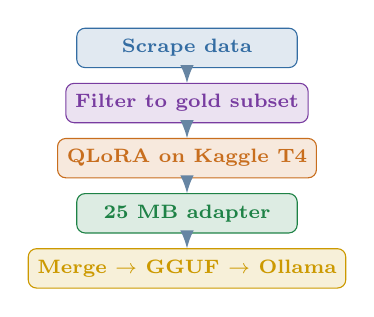
\begin{tikzpicture}[font=\scriptsize, every node/.style={align=center}]
          \def\bw{2.8cm}\def\bh{0.5cm}
          \foreach \i/\col/\lbl in {
            5/moduleblue/Scrape data,
            4/modulepurple/Filter to gold subset,
            3/moduleorange/QLoRA on Kaggle T4,
            2/accentgreen/25~MB adapter,
            1/sfaxgold/Merge $\to$ GGUF $\to$ Ollama}
          {
            \node[fill=\col!15, draw=\col, rounded corners=3pt,
                  minimum width=\bw, minimum height=\bh, font=\scriptsize\bfseries,
                  text=\col] at (0,\i*0.7) {\lbl};
          }
          \foreach \i in {2,3,4,5}
            \draw[->, >=Latex, sfaxblue!60, thick] (0,\i*0.7-0.25) -- (0,\i*0.7-0.45);
        \end{tikzpicture}
      \end{center}
    \end{column}
  \end{columns}
\end{frame}

% ================================================================
\section{Research Lineage}
% ================================================================

\begin{frame}{How the research line evolved}
  \centering
  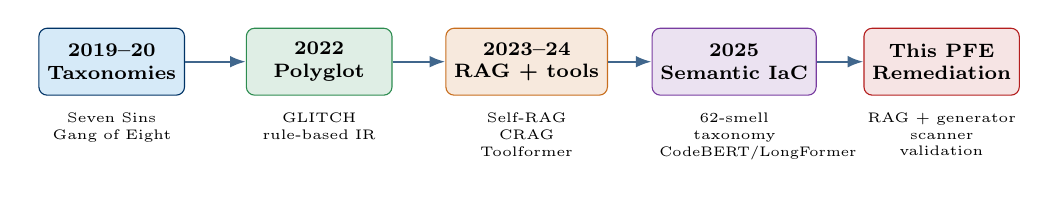
\begin{tikzpicture}[
      font=\scriptsize,
      x=1.55cm,
      y=1cm,
      milestone/.style={
        draw, rounded corners=3pt, align=center,
        minimum width=1.85cm, minimum height=0.85cm,
        inner sep=3pt, font=\scriptsize\bfseries
      },
      detail/.style={font=\tiny, align=center, text width=1.9cm},
      arrow/.style={-{Latex[length=2mm]}, thick, sfaxblue!75}
    ]
    \node[milestone, fill=sfaxlightblue, draw=sfaxblue] (s1) at (0,0)
      {2019--20\\Taxonomies};
    \node[detail, below=1mm of s1] {Seven Sins\\Gang of Eight};

    \node[milestone, fill=modulegreen!15, draw=modulegreen] (s2) at (1.7,0)
      {2022\\Polyglot};
    \node[detail, below=1mm of s2] {GLITCH\\rule-based IR};

    \node[milestone, fill=moduleorange!15, draw=moduleorange] (s3) at (3.4,0)
      {2023--24\\RAG + tools};
    \node[detail, below=1mm of s3] {Self-RAG\\CRAG\\Toolformer};

    \node[milestone, fill=modulepurple!15, draw=modulepurple] (s4) at (5.1,0)
      {2025\\Semantic IaC};
    \node[detail, below=1mm of s4] {62-smell taxonomy\\CodeBERT/LongFormer};

    \node[milestone, fill=accentred!12, draw=accentred] (s5) at (6.8,0)
      {This PFE\\Remediation};
    \node[detail, below=1mm of s5] {RAG + generator\\scanner validation};

    \foreach \a/\b in {s1/s2,s2/s3,s3/s4,s4/s5}
      \draw[arrow] (\a) -- (\b);
  \end{tikzpicture}

  \vspace{1.0em}
  \begin{columns}[T]
    \begin{column}{0.47\textwidth}
      \begin{block}{What prior work gives us}
        \scriptsize
        \begin{itemize}
          \item A vocabulary of IaC security smells.
          \item Static and semantic detectors.
          \item RAG/self-verification patterns.
        \end{itemize}
      \end{block}
    \end{column}
    \begin{column}{0.47\textwidth}
      \begin{exampleblock}{Where this thesis is positioned}
        \scriptsize
        Move from \textbf{detecting} smells to generating and validating
        concrete IaC remediations inside an agentic loop.
      \end{exampleblock}
    \end{column}
  \end{columns}
\end{frame}

% ================================================================
\section{Positioning}
% ================================================================

\begin{frame}{Where this work fits in the project}
  \begin{columns}[T]
    \begin{column}{0.55\textwidth}
      \begin{block}{Agentic IaC security framework (Rapport 2)}
        Seven modules cooperating under a central orchestrator:
        \begin{itemize}\scriptsize
          \item Contextual Analyzer
          \item Knowledge Base + RAG Retriever
          \item \textbf{Fix Generator} \faArrowRight\ this work
          \item External Validator (Checkov + KICS)
          \item Patch Formatter \& Explanation
        \end{itemize}
      \end{block}
      \begin{alertblock}{Why touch the Fix Generator now?}
        \scriptsize
        It is the \emph{only} module whose quality depends on the
        underlying LLM rather than on deterministic software.
      \end{alertblock}
    \end{column}
    \begin{column}{0.42\textwidth}
      \begin{exampleblock}{Two informal observations on the baseline}
        \scriptsize
        \begin{itemize}
          \item Off-the-shelf small LLMs (Gemma-3-4B, Gemma-4-e2B)
                produce plausible fixes but do not always target the
                declared CWE.
          \item On CPU, Gemma-4-e2B $\approx$ \textbf{320 s / fix}
                $\Rightarrow$ full eval with self-consistency is
                impractical on current hardware.
        \end{itemize}
      \end{exampleblock}
      \begin{block}{This report}
        \scriptsize
        A first, preliminary attempt to fine-tune a small open-weight
        model on our own scraped data.
      \end{block}
    \end{column}
  \end{columns}
\end{frame}

\begin{frame}{Scope of this experiment}
  \begin{block}{What this is}
    A \textbf{first, exploratory} run to validate the pipeline end-to-end.
  \end{block}
  \begin{columns}[T]
    \begin{column}{0.48\textwidth}
      \begin{exampleblock}{In scope}
        \scriptsize
        \begin{itemize}
          \item Small base model ($\approx$\,2\,B params)
          \item Subset of the scraped data (3{,}227 train)
          \item 1 epoch, 1 random seed
          \item 1 prompt template
          \item Qualitative check on \textbf{n\,=\,3} samples
          \item Kaggle free T4 GPU
        \end{itemize}
      \end{exampleblock}
    \end{column}
    \begin{column}{0.48\textwidth}
      \begin{alertblock}{Out of scope}
        \scriptsize
        \begin{itemize}
          \item No hyperparameter search
          \item No comparison against baselines
          \item No downstream task-level metric
                (scanner pass-rate)
          \item No multi-seed variance estimate
          \item No claim of competitive performance
        \end{itemize}
      \end{alertblock}
    \end{column}
  \end{columns}
  \vspace{0.3em}
  \begin{center}
    \scriptsize\color{sfaxblue}\itshape
    Goal: demonstrate that the pipeline works and surface the obstacles
    that block a scaled experiment.
  \end{center}
\end{frame}

% ================================================================
\section{Background: LoRA, QLoRA, SFT}
% ================================================================

\begin{frame}{LoRA in one slide}
  \begin{columns}[T]
    \begin{column}{0.55\textwidth}
      \begin{block}{Core idea}
        \scriptsize
        Freeze the pretrained weights $W_0 \in \mathbb{R}^{d\times k}$
        and learn a low-rank update
        \[
          \Delta W = B A,\quad
          B\!\in\!\mathbb{R}^{d\times r},\;
          A\!\in\!\mathbb{R}^{r\times k},\;
          r \ll \min(d,k).
        \]
        Effective weight at inference: $W = W_0 + \Delta W$.
      \end{block}
      \begin{exampleblock}{For Gemma-2-2B, $r\,=\,16$ on attention only}
        \scriptsize
        \begin{itemize}
          \item Trainable params: \textbf{9.27\,M} out of 2.6\,B
                ($\approx$\,0.35\,\%)
          \item Adapter file: \textbf{25\,MB} (vs.\ 5\,GB full model)
        \end{itemize}
      \end{exampleblock}
    \end{column}
    \begin{column}{0.42\textwidth}
      \begin{center}
        \begin{tikzpicture}[
            font=\scriptsize,
            arr/.style={-{Latex[length=2mm]}, line width=0.7pt},
          ]
          % --- input ---
          \node[font=\scriptsize\bfseries] (x) at (0,0) {$x$};

          % --- fork point (invisible) ---
          \coordinate[right=0.9cm of x] (fork);

          % --- frozen W0 (large ~square, d×k both big) ---
          \node[draw=sfaxblue!85, fill=sfaxblue!12, rounded corners=2pt,
                minimum width=1.45cm, minimum height=1.0cm,
                font=\scriptsize\bfseries, inner sep=4pt,
                right=0.5cm of fork, yshift=0.95cm] (w0) {\faLock~$W_0$};

          % --- A: wide pancake (r×k, r is tiny) ---
          \node[draw=moduleorange!80, fill=moduleorange!12, rounded corners=2pt,
                minimum width=1.8cm, minimum height=0.30cm,
                font=\scriptsize\bfseries, inner sep=2pt,
                right=1.1cm of fork, yshift=-0.75cm] (a) {$A$};

          % --- B: tall pillar (d×r, r is tiny) ---
          \node[draw=moduleorange!80, fill=moduleorange!12, rounded corners=2pt,
                minimum width=0.38cm, minimum height=1.15cm,
                font=\scriptsize\bfseries, inner sep=2pt,
                right=0.15cm of a] (b) {$B$};

          % --- dashed box around A,B ---
          \begin{scope}[on background layer]
            \node[draw=moduleorange!70, dashed, rounded corners=3pt,
                  inner xsep=4pt, inner ysep=7pt,
                  fit=(a)(b),
                  label={[text=moduleorange!85,font=\tiny\bfseries]south:trainable}] {};
          \end{scope}

          % --- sum circle ---
          \node[circle, draw=sfaxdark, fill=white, inner sep=0pt,
                minimum size=0.50cm, font=\bfseries,
                right=0.45cm of b] (plus) {$\Sigma$};

          % --- output ---
          \node[font=\scriptsize\bfseries, right=0.3cm of plus] (h) {$h$};

          % --- arrows ---
          \draw[arr, sfaxblue!70] (x.east) -- (fork) |- (w0.west);
          \draw[arr, sfaxblue!70] (w0.east) -| (plus.north);
          \draw[arr, moduleorange!80] (x.east) -- (fork) |- (a.west);
          \draw[arr, moduleorange!80] (a.east) -- (b.west);
          \draw[arr, moduleorange!80] (b.east) -- (plus.west);
          \draw[arr, sfaxdark] (plus.east) -- (h.west);

          % --- dimension labels on matrices ---
          \node[font=\tiny\itshape, text=sfaxblue!75, below=0.02cm of w0]
            {$\mathbb{R}^{d \times k}$};

          % --- dimension callouts for the low-rank bottleneck ---
          % k above A (the wide dimension of the pancake)
          \draw[moduleorange!60, line width=0.4pt,
                {Latex[length=1.5mm]}-{Latex[length=1.5mm]}]
                ($(a.north west)+(0,0.15)$) -- ($(a.north east)+(0,0.15)$);
          \node[font=\tiny, text=moduleorange!80, above=0.02cm]
                at ($(a.north)!0.5!(a.north east)+(0,0.15)$) {$k$};

          % r above B (the narrow dimension)
          \draw[moduleorange!60, line width=0.4pt,
                {Latex[length=1.5mm]}-{Latex[length=1.5mm]}]
                ($(b.north west)+(-0.05,0.15)$) -- ($(b.north east)+(0.05,0.15)$);
          \node[font=\tiny, text=moduleorange!80, above=0.02cm]
                at ($(b.north)!0.5!(b.north east)+(0,0.15)$) {$r$};

          % d on the left side of W0
          \draw[sfaxblue!50, line width=0.4pt,
                {Latex[length=1.5mm]}-{Latex[length=1.5mm]}]
                ($(w0.north west)+(-0.15,0)$) -- ($(w0.south west)+(-0.15,0)$);
          \node[font=\tiny, text=sfaxblue!70, left=0.02cm]
                at ($(w0.west)!0.5!(w0.south west)+(-0.15,0)$) {$d$};

          % d on the right side of B
          \draw[moduleorange!60, line width=0.4pt,
                {Latex[length=1.5mm]}-{Latex[length=1.5mm]}]
                ($(b.north east)+(0.10,0)$) -- ($(b.south east)+(0.10,0)$);
          \node[font=\tiny, text=moduleorange!80, right=0.02cm]
                at ($(b.east)!0.5!(b.south east)+(0.10,0)$) {$d$};

          % --- key formula ---
          \node[font=\tiny, text=sfaxdark, below=1.35cm of a, align=center]
            {$W = W_0 + BA,\qquad r \ll d{,}k$};
        \end{tikzpicture}
      \end{center}
    \end{column}
  \end{columns}
\end{frame}

\begin{frame}{QLoRA and supervised fine-tuning}
  \begin{columns}[T]
    \begin{column}{0.48\textwidth}
      \begin{block}{QLoRA = LoRA on 4-bit base}
        \scriptsize
        \begin{itemize}
          \item Base weights stored in \textbf{NF4} (4-bit NormalFloat)
                with double-quantised scales
          \item Tiles decompressed on the fly for forward pass
          \item Activations in fp16, gradients routed \emph{only}
                through $A$/$B$
          \item Memory footprint for 2-B model:
                $\approx$\,5\,GB fp16 $\to$ \textbf{$\approx$\,1.6\,GB NF4}
        \end{itemize}
      \end{block}
      \begin{exampleblock}{Consequence}
        \scriptsize
        A 2-B model becomes trainable on a \textbf{single 16\,GB T4}
        --- exactly what Kaggle's free tier offers.
      \end{exampleblock}
    \end{column}
    \begin{column}{0.48\textwidth}
      \begin{block}{Supervised fine-tuning (SFT) for code repair}
        \scriptsize
        Task: given a \emph{detected smell} and an \emph{insecure snippet},
        output a \emph{fixed snippet}.
        \begin{itemize}
          \item Standard causal-LM cross-entropy loss
          \item Loss computed \textbf{only on the model turn}
                (the fix tokens), prompt tokens are masked
          \item Closer to code-to-code translation than to free
                code generation
        \end{itemize}
      \end{block}
      \begin{alertblock}{Why SFT (and not RL / preference optimisation) here?}
        \scriptsize
        We have before/after pairs, not ranked preferences.
        SFT matches the data we already have.
      \end{alertblock}
    \end{column}
  \end{columns}
\end{frame}

% ================================================================
\section{Dataset}
% ================================================================

\begin{frame}{Dataset origin: our own scraper}
  \begin{columns}[T]
    \begin{column}{0.52\textwidth}
      \begin{block}{Five complementary sources}
        \scriptsize
        \begin{itemize}
          \item GitHub \textbf{commit search} with date-window
                partitioning (to bypass the 1{,}000-result cap)
          \item \textbf{GHArchive} hourly event dumps
                (bypasses the Search API quota)
          \item \textbf{Scanner test suites} (Checkov / KICS / tfsec):
                paired ``failed'' / ``passed'' examples
          \item \textbf{Known vulnerable repos}:
                TerraGoat, Kubernetes-Goat, WrongSecrets
          \item \textbf{Scanner-validated labels}: Checkov + tfsec +
                KICS rerun on every record
        \end{itemize}
      \end{block}
    \end{column}
    \begin{column}{0.46\textwidth}
      \begin{exampleblock}{Dataset v1 --- headline figures}
        \scriptsize
        \begin{tabular}{@{}lr@{}}
          \toprule
          Total records (dedup)       & 31{,}748 \\
          With a fix                  & 16{,}362 \\
          Scanner-validated           & 10{,}791 \\
          Source repositories         & $>$\,2{,}000 \\
          Smell types                 & 18 \\
          \bottomrule
        \end{tabular}
      \end{exampleblock}
      \begin{block}{Tool mix (v1 raw)}
        \scriptsize
        Terraform 50\,\% \textbullet\ Kubernetes 28\,\% \textbullet\
        Ansible 13\,\% \textbullet\ Docker 7\,\% \textbullet\
        CloudFormation 1.5\,\%
      \end{block}
    \end{column}
  \end{columns}
\end{frame}

\begin{frame}{From 31{,}748 raw records to a 3{,}227-record training set}
  \centering\small
  \begin{tabular}{lrr}
    \toprule
    \textbf{Filter} & \textbf{Remaining} & \textbf{Share of input} \\
    \midrule
    All validated records                                            & 31{,}748          & 100.0\,\% \\
    \texttt{has\_fix} = True                                         & 16{,}362          & 51.5\,\% \\
    Scanner-validated only                                           & $\sim$10{,}791    & 34.0\,\% \\
    Non-empty \texttt{code\_before} and \texttt{code\_after}         & $\sim$10{,}500    & ---      \\
    Combined length $<$ 8{,}000 chars                                & $\sim$5{,}500     & ---      \\
    Non-noop fix (\texttt{before} $\neq$ \texttt{after})             & \textbf{4{,}050}  & 12.76\,\% \\
    Pre-existing train split (80\,\%)                                & \textbf{3{,}227}  & ---      \\
    \bottomrule
  \end{tabular}

  \vspace{0.6em}
  \begin{columns}[T]
    \begin{column}{0.49\textwidth}
      \begin{exampleblock}{Gold subset --- better-balanced tool mix}
        \scriptsize
        Docker 32\,\% \textbullet\ Terraform 30\,\% \textbullet\
        Kubernetes 30\,\% \textbullet\ CloudFormation 5\,\% \textbullet\
        Ansible 3\,\%
      \end{exampleblock}
    \end{column}
    \begin{column}{0.49\textwidth}
      \begin{alertblock}{Caveat --- this is a deliberate subset}
        \scriptsize
        We chose the \textbf{strictest} filter for this first run.
        A larger (but noisier) corpus of up to $\sim$\,10{,}791 records
        is available and has not been used yet.
      \end{alertblock}
    \end{column}
  \end{columns}
\end{frame}

\begin{frame}[fragile]{Training sample format}
  \begin{block}{Slim JSON record}
  \begin{lstlisting}[basicstyle=\ttfamily\scriptsize]
  {
    "id": "a1b2c3d4",
    "iac_tool": "terraform",
    "smell_types": ["hardcoded_credential", "overly_permissive_cidr"],
    "cwes": ["CWE-798", "CWE-732"],
    "code_before": "resource aws_s3_bucket ...",
    "code_after":  "resource aws_s3_bucket ...",
    "split": "train"
  }
  \end{lstlisting}
  \end{block}
  \begin{exampleblock}{Rendered at training time via the Gemma-2 chat template}
  \begin{lstlisting}[basicstyle=\ttfamily\scriptsize]
  You are a security expert specializing in Infrastructure as Code (IaC).
  Fix the following {iac_tool} script. Detected smells: {smells}.
  Return ONLY the corrected script, no explanation.

  ```
  {code_before}
  ```
  \end{lstlisting}
  \end{exampleblock}
\end{frame}

% ================================================================
\section{Method}
% ================================================================

\begin{frame}{Base model: Gemma-2-2B-IT}
  \centering\small
  \begin{tabular}{lllp{4.2cm}}
    \toprule
    \textbf{Model} & \textbf{Size} & \textbf{Gated} & \textbf{Remark} \\
    \midrule
    google/codegemma-2b-it           & 2\,B & Yes & Code-specialised \\
    \rowcolor{sfaxlightblue}
    \textbf{google/gemma-2-2b-it}    & 2\,B & Yes & \textbf{Chosen} --- matches Ollama stack \\
    Qwen/Qwen2.5-Coder-3B-Instruct   & 3\,B & No  & Stronger code model, non-gated \\
    bigcode/starcoder2-3b            & 3\,B & No  & No chat template \\
    \bottomrule
  \end{tabular}

  \vspace{0.6em}
  \begin{columns}[T]
    \begin{column}{0.48\textwidth}
      \begin{block}{Reasons for this choice}
        \scriptsize
        \begin{itemize}
          \item Same family as our local Ollama stack
                (Gemma-3-4B, Gemma-4-e2B) --- no new architecture
          \item Published chat template that maps onto our
                instruction/response pair
          \item Smallest Gemma-2: VRAM headroom on T4, a few hours per run
        \end{itemize}
      \end{block}
    \end{column}
    \begin{column}{0.48\textwidth}
      \begin{alertblock}{This is a pragmatic choice, not an optimum}
        \scriptsize
        No systematic model comparison is in scope here.
        Larger candidates (3\,B, 7\,B, 9\,B) are deferred to a
        later iteration.
      \end{alertblock}
    \end{column}
  \end{columns}
\end{frame}

\begin{frame}{QLoRA configuration}
  \centering\scriptsize
  \begin{tabular}{ll}
    \toprule
    \textbf{Parameter} & \textbf{Value} \\
    \midrule
    Quantisation          & 4-bit NF4 (double-quant, fp16 compute) \\
    LoRA rank $r$         & 16 \\
    LoRA $\alpha$         & 32 \\
    LoRA dropout          & 0.05 \\
    Target modules        & \texttt{q\_proj}, \texttt{k\_proj}, \texttt{v\_proj}, \texttt{o\_proj} \\
    Trainable params      & 9{,}273{,}344  (0.35\,\%) \\
    Learning rate         & $2 \times 10^{-4}$ \\
    Scheduler / warmup    & Cosine / 3\,\% \\
    Effective batch       & 8  (1 $\times$ 8 grad.\ accumulation) \\
    Epochs                & \textbf{1} \\
    Optimiser             & Paged AdamW 8-bit \\
    Max seq.\ length      & 2{,}048 tokens \\
    Precision             & fp16 (bf16 unavailable on T4) \\
    Gradient checkpointing& Enabled (non-reentrant) \\
    Random seed           & 42 \\
    \bottomrule
  \end{tabular}

  \vspace{0.5em}
  \begin{center}
    \scriptsize\color{sfaxblue}\itshape
    Values copied from published recipes --- no hyperparameter search was
    performed in this first run.
  \end{center}
\end{frame}

% ================================================================
\section{Execution on Kaggle}
% ================================================================

\begin{frame}{Kaggle environment}
  \begin{columns}[T]
    \begin{column}{0.5\textwidth}
      \begin{block}{Runtime}
        \scriptsize
        \begin{itemize}
          \item Accelerator: NVIDIA \textbf{T4 (16\,GB)}
          \item CUDA: 12.8
          \item Python: 3.12
          \item Session limit: 9\,h per notebook
          \item Internet: on (to fetch base model)
          \item Attachments: 2 custom Kaggle datasets
                (scripts + filtered corpus)
        \end{itemize}
      \end{block}
    \end{column}
    \begin{column}{0.48\textwidth}
      \begin{alertblock}{Three issues encountered (for reproducibility)}
        \scriptsize
        \begin{itemize}
          \item \textbf{403 Forbidden} on Gemma-2 \\
                $\to$ accept license on HF page
          \item \texttt{bitsandbytes} 0.43.3 lacks CUDA 12.8 binary \\
                $\to$ upgrade to 0.49.2 in-place
          \item Kernel restart wipes env vars \\
                $\to$ re-run the HF-token cell first
        \end{itemize}
      \end{alertblock}
    \end{column}
  \end{columns}
\end{frame}

\begin{frame}[fragile]{The five Kaggle cells (summary)}
  % compact styles for this slide only
  \lstdefinestyle{kcell}{style=shell,
      basicstyle=\ttfamily\fontsize{5.8}{6.6}\selectfont,
      aboveskip=1pt, belowskip=1pt, xleftmargin=2pt, xrightmargin=2pt,
      framexleftmargin=1pt, framexrightmargin=1pt}
  \setbeamertemplate{blocks}[rounded][shadow=false]
  \begin{columns}[T]
    \begin{column}{0.48\textwidth}
      \begin{block}{\faCog\ Cell 1 --- Install deps}
      \begin{lstlisting}[style=kcell]
!pip install -q -U transformers==4.44.2 \
  datasets==2.21.0 peft==0.12.0 \
  accelerate==0.34.2 bitsandbytes==0.43.3 \
  trl==0.10.1
!pip install -q -U bitsandbytes
      \end{lstlisting}
      \end{block}
      \vspace{-2mm}
      \begin{block}{\faKey\ Cell 2 --- Expose HF token}
      \begin{lstlisting}[style=kcell]
from kaggle_secrets import UserSecretsClient
os.environ["HF_TOKEN"] = \
  UserSecretsClient().get_secret("HF_TOKEN")
      \end{lstlisting}
      \end{block}
      \vspace{-2mm}
      \begin{block}{\faFlask\ Cell 3 --- Smoke test (200 samples)}
      \begin{lstlisting}[style=kcell]
!python 02_train_qlora.py \
  --model google/gemma-2-2b-it \
  --data-dir .../data \
  --output-dir /kaggle/working/lora_smoke \
  --epochs 1 --max-train-samples 200
      \end{lstlisting}
      \end{block}
    \end{column}
    \begin{column}{0.48\textwidth}
      \begin{exampleblock}{\faRocket\ Cell 4 --- Full training (1 epoch)}
      \begin{lstlisting}[style=kcell]
!python 02_train_qlora.py \
  --model google/gemma-2-2b-it \
  --data-dir .../data \
  --output-dir /kaggle/working/lora_out \
  --epochs 1 --batch-size 1 \
  --grad-accum 8 --lr 2e-4
      \end{lstlisting}
      \end{exampleblock}
      \vspace{-2mm}
      \begin{block}{\faSearch\ Cell 5 --- Inference check}
      \begin{lstlisting}[style=kcell]
!python 03_inference.py \
  --model google/gemma-2-2b-it \
  --adapter /kaggle/working/lora_out \
  --input-file .../test.jsonl \
  --n-samples 3
      \end{lstlisting}
      \end{block}
      \vspace{-2mm}
      \begin{alertblock}{Smoke test is a sanity check, not a curve}
      \scriptsize
      Produces a single final loss, not a learning curve; only the full
      run yields a per-step loss trajectory.
      \end{alertblock}
    \end{column}
  \end{columns}
\end{frame}

% ================================================================
\section{Results}
% ================================================================

\begin{frame}{Training metrics (single run, seed 42)}
  \begin{columns}[T]
    \begin{column}{0.48\textwidth}
      \centering\scriptsize
      \begin{tabular}{lr}
        \toprule
        \textbf{Metric} & \textbf{Value} \\
        \midrule
        Optimisation steps          & 403 \\
        Training wall-clock         & 1\,h\,47\,min \\
        Evaluation wall-clock       & 218\,s \\
        Average step time           & 15.94\,s \\
        Training throughput         & 0.502 samples/s \\
        Final training loss         & \textbf{0.528} \\
        Final evaluation loss       & \textbf{0.467} \\
        Adapter size (safetensors)  & 25.6\,MB \\
        \bottomrule
      \end{tabular}
    \end{column}
    \begin{column}{0.48\textwidth}
      \begin{alertblock}{How to read these numbers}
        \scriptsize
        \begin{itemize}
          \item \textbf{One run, one seed} --- no confidence interval.
          \item Absolute loss is tokeniser-dependent; not directly
                comparable across models or papers.
          \item \texttt{eval\_loss < train\_loss} is consistent with
                \emph{no overfitting} after 1 epoch, but can also be
                explained by:
            \begin{itemize}\tiny
              \item training loss averaged over high-loss early steps,
              \item LoRA dropout on at train, off at eval,
              \item eval split possibly slightly easier.
            \end{itemize}
          \item \textbf{Not} evidence of superior generalisation.
        \end{itemize}
      \end{alertblock}
    \end{column}
  \end{columns}
\end{frame}

\begin{frame}{Qualitative inspection --- 3 held-out test samples}
  \centering\scriptsize
  \begin{tabular}{cp{2.2cm}p{3.8cm}p{4.2cm}}
    \toprule
    \# & \textbf{Declared smells} & \textbf{Human ground truth} & \textbf{Fine-tuned model output} \\
    \midrule
    1 & \texttt{apt\_no\_install\_recommends}, \texttt{unpinned\_base\_image} (Docker)
      & Version bump ATMOS\,1.210\,$\to$\,1.214 --- \emph{does not address the declared smell}
      & Adds \texttt{--allow-downgrades}, creates non-root user \texttt{appuser}
        --- sensible but unrelated hardening \\
    \addlinespace[2pt]
    2 & \texttt{uri\_credentials} (Terraform)
      & Changes \texttt{recovery\_window\_in\_days 0\,$\to$\,7}
        --- unrelated
      & Adds IRSA / IAM scaffolding, keeps 0 --- does not target URI credentials \\
    \addlinespace[2pt]
    3 & \texttt{unpinned\_base\_image} (Docker)
      & Pins a Go image by \texttt{sha256:}\ digest (\checkmark{} real pin)
      & Does not pin; performs unrelated hardening (\texttt{apt-get upgrade}, labels)\\
    \bottomrule
  \end{tabular}

  \vspace{0.5em}
  \begin{columns}[T]
    \begin{column}{0.49\textwidth}
      \begin{exampleblock}{What we see (with $n\,=\,3$ caveat)}
      \scriptsize
      \begin{itemize}
        \item Output is syntactically well-formed on these 3 cases.
        \item Contains idiomatic hardening patterns.
      \end{itemize}
      \end{exampleblock}
    \end{column}
    \begin{column}{0.49\textwidth}
      \begin{alertblock}{What we see (worrying)}
      \scriptsize
      \begin{itemize}
        \item Model \emph{and human ground truth} often fail to
              address the declared smell.
        \item \textbf{The label itself is noisy.}
      \end{itemize}
      \end{alertblock}
    \end{column}
  \end{columns}
\end{frame}

% ================================================================
\section{Discussion}
% ================================================================

\begin{frame}{Label noise is the binding constraint}
  \begin{columns}[T]
    \begin{column}{0.55\textwidth}
      \begin{alertblock}{The problem}
        \scriptsize
        Commit-scraped pairs are at \textbf{file granularity}, but a
        single commit may bundle several unrelated modifications.
        \begin{itemize}
          \item Regex classifier infers the smell from the
                \emph{commit message} (not the diff).
          \item Scanner validation only confirms that \texttt{code\_before}
                was vulnerable --- not that the \emph{removed lines}
                address that vulnerability.
        \end{itemize}
      \end{alertblock}
      \begin{block}{Practical consequence}
        \scriptsize
        Training signal = average of (a)~genuine smell$\to$patch pairs
        and (b)~unrelated refactors that happen to coexist in a
        ``fix: security'' commit.\\
        The model can only learn the distribution of
        \emph{``things that look like fix commits''}.
      \end{block}
    \end{column}
    \begin{column}{0.42\textwidth}
      \begin{exampleblock}{Two remediations (for next iteration)}
        \scriptsize
        \begin{enumerate}
          \item \textbf{Hunk-level filter}: keep only records whose
                \emph{diff} regex-matches the declared smell.
          \item \textbf{Scanner-fixture-only corpus}: $\sim$\,1{,}850
                Checkov + KICS test pairs where the smell is,
                by construction, what the scanner flags.
        \end{enumerate}
      \end{exampleblock}
    \end{column}
  \end{columns}
\end{frame}

\begin{frame}{Limitations and threats to validity}
  \begin{columns}[T]
    \begin{column}{0.48\textwidth}
      \begin{alertblock}{Experimental limitations}
        \scriptsize
        \begin{itemize}
          \item \textbf{Small model} (2\,B parameters)
          \item \textbf{Subset of the data} (3{,}227 train)
          \item \textbf{1 epoch}, \textbf{1 seed}, \textbf{1 prompt template}
          \item No hyperparameter search
          \item No downstream (scanner-level) metric
          \item Qualitative look at only \textbf{n\,=\,3} samples
        \end{itemize}
      \end{alertblock}
    \end{column}
    \begin{column}{0.48\textwidth}
      \begin{block}{Threats to validity}
        \scriptsize
        \begin{itemize}
          \item \textbf{External}: dataset skewed toward public
                Docker/Kubernetes repos.
          \item \textbf{Construct}: ``smell'' = ``pattern detected by
                Checkov/tfsec/KICS''; excludes business-logic flaws.
          \item \textbf{Internal}: single run, no variance estimate.
        \end{itemize}
      \end{block}
      \begin{exampleblock}{What this run \emph{does} demonstrate}
        \scriptsize
        The end-to-end pipeline runs within Kaggle's free GPU tier,
        produces a coherent 25\,MB adapter, and surfaces a
        \emph{measurable} obstacle to improvement: label noise.
      \end{exampleblock}
    \end{column}
  \end{columns}
\end{frame}

% ================================================================
\section{Next Steps}
% ================================================================

\begin{frame}{Integration path: adapter $\to$ Ollama}
  \centering
  \resizebox{0.96\textwidth}{!}{%
  \begin{tikzpicture}[
      every node/.style={font=\scriptsize},
      box/.style={draw, rounded corners=3pt, minimum width=2.00cm,
                  minimum height=1.10cm, align=center, font=\scriptsize,
                  inner sep=2pt,
                  drop shadow={shadow blur steps=4,opacity=0.22}},
      input/.style={box, fill=sfaxlightblue, draw=sfaxblue!70,
                    minimum width=2.00cm},
      arrow/.style={-{Latex[length=2.3mm]}, thick, sfaxblue!85},
      steplbl/.style={font=\tiny\bfseries, text=sfaxdark,
                      fill=sfaxgold!30, rounded corners=2pt,
                      inner xsep=2.5pt, inner ysep=1.5pt,
                      draw=sfaxgold!70, line width=0.3pt},
      fmt/.style={font=\tiny\itshape, text=sfaxblue!80}
    ]
    % --- inputs (left column, stacked) ---
    \node[input] (base)
      {\textbf{Gemma-2-2B-IT}\\\tiny base weights\\\tiny fp16 $\cdot$ $\sim$\,5\,GB};
    \node[input, below=5mm of base, fill=moduleorange!15, draw=moduleorange!80] (adapter)
      {\textbf{LoRA adapter}\\\tiny $A,B$ matrices, $r{=}16$\\\tiny safetensors $\cdot$ 25\,MB};

    % --- pipeline (horizontal, right of inputs) ---
    \node[box, fill=modulepurple!18, draw=modulepurple!80,
          right=1.55cm of base.east, yshift=-10mm] (merged)
      {\textbf{Merged HF model}\\\tiny $W_0 + BA$ (in-place)\\\tiny safetensors $\cdot$ $\sim$\,5\,GB};
    \node[box, right=1.55cm of merged, fill=moduleblue!18, draw=moduleblue!80] (gguf)
      {\textbf{GGUF Q4\_K\_M}\\\tiny 4-bit k-quant\\\tiny single file $\cdot$ $\sim$\,1.5\,GB};
    \node[box, right=1.55cm of gguf, fill=accentgreen!18, draw=accentgreen!80] (ollama)
      {\textbf{Ollama model}\\\tiny registered locally\\\tiny \texttt{iac-fixer:latest}};

    % --- downstream framework consumer ---
    \node[box, below=7mm of ollama, fill=sfaxgold!25, draw=sfaxgold!90,
          minimum width=2.35cm] (agent)
      {\faRobot\ \textbf{FixGenerator}\\\tiny agent module\\\tiny reads \texttt{OLLAMA\_MODEL}};

    % --- arrows: inputs converge to merged ---
    \draw[arrow] (base.east)    -| (merged.west);
    \draw[arrow] (adapter.east) -| (merged.west);

    % --- step label for the merge step ---
    \node[steplbl] at ($(base.east)!0.5!(merged.west)+(0,0.55)$)
      {04\_merge\_adapter};
    \node[fmt]    at ($(base.east)!0.5!(merged.west)+(0,0.25)$)
      {PEFT merge};

    % --- horizontal pipeline arrows ---
    \draw[arrow] (merged.east) -- (gguf.west);
    \node[steplbl] at ($(merged.east)!0.5!(gguf.west)+(0,0.32)$)
      {05\_to\_gguf};
    \node[fmt]    at ($(merged.east)!0.5!(gguf.west)+(0,-0.30)$)
      {llama.cpp};

    \draw[arrow] (gguf.east) -- (ollama.west);
    \node[steplbl] at ($(gguf.east)!0.5!(ollama.west)+(0,0.32)$)
      {06\_ollama};
    \node[fmt]    at ($(gguf.east)!0.5!(ollama.west)+(0,-0.30)$)
      {Modelfile};

    % --- final consumer arrow ---
    \draw[arrow] (ollama.south) -- (agent.north);
    \node[fmt] at ($(ollama.south)!0.5!(agent.north)+(0.9,0)$)
      {\texttt{.env} switch};
  \end{tikzpicture}%
  }

  \vspace{0.2em}
  \begin{columns}[T]
    \begin{column}{0.49\textwidth}
      \begin{block}{Three new scripts added to the repo}
        \scriptsize
        \begin{itemize}
          \item \texttt{04\_merge\_adapter.py}
                --- \texttt{PeftModel.merge\_and\_unload()}
          \item \texttt{05\_convert\_to\_gguf.sh}
                --- llama.cpp \texttt{convert\_hf\_to\_gguf.py} + \texttt{llama-quantize}
          \item \texttt{06\_ollama\_create.sh}
                --- Modelfile + \texttt{ollama create iac-fixer}
        \end{itemize}
      \end{block}
    \end{column}
    \begin{column}{0.49\textwidth}
      \begin{exampleblock}{Framework change required: one line}
        \scriptsize
        Set \texttt{OLLAMA\_MODEL=iac-fixer} in \texttt{.env}.
        \texttt{FixGenerator} already reads the backend from env vars, so
        no code change is needed downstream.
      \end{exampleblock}
    \end{column}
  \end{columns}
\end{frame}

\begin{frame}{Config B evaluation --- the remaining deliverable}
  \begin{block}{Evaluation plan (from Rapport 2, Chapter 6)}
    \scriptsize
    \begin{tabular}{lll}
      \toprule
      \textbf{Config} & \textbf{Composition} & \textbf{Status} \\
      \midrule
      A & Checkov alone                                              & \textbf{Measured}. F1=0.132, P=0.084, R=0.304 \\
      \rowcolor{sfaxgold!15}
      B & Analyzer + fine-tuned LLM + validator (full pipeline)      & \textbf{Pending} --- this work enables it \\
      C & Config B + self-consistency (N=5) + iterative retrieval    & Deferred \\
      \bottomrule
    \end{tabular}
  \end{block}
  \begin{columns}[T]
    \begin{column}{0.48\textwidth}
      \begin{exampleblock}{Primary metrics (consistent with Rapport 2)}
        \scriptsize
        \begin{itemize}
          \item Patch Validity Rate
          \item Smell Elimination Rate
          \item No-New-Issues Rate
          \item Macro-F1 over the ground-truth smell set
        \end{itemize}
      \end{exampleblock}
    \end{column}
    \begin{column}{0.48\textwidth}
      \begin{alertblock}{Sequencing}
        \scriptsize
        \begin{enumerate}
          \item Merge adapter locally
          \item GGUF + Ollama registration
          \item Run \texttt{scripts/evaluate.py}
                on the labelled 16-file benchmark
          \item Compare Config A vs B
        \end{enumerate}
      \end{alertblock}
    \end{column}
  \end{columns}
\end{frame}

\begin{frame}{Roadmap beyond Config B}
  \begin{columns}[T]
    \begin{column}{0.32\textwidth}
      \begin{block}{Data}
        \scriptsize
        \begin{itemize}
          \item Hunk-level diff filter
          \item Scanner-fixture-only corpus
          \item Extend scraper v2 with hunk-level classifier
        \end{itemize}
      \end{block}
    \end{column}
    \begin{column}{0.32\textwidth}
      \begin{block}{Model}
        \scriptsize
        \begin{itemize}
          \item Try Qwen2.5-Coder-3B (non-gated, stronger on code)
          \item 2--3 epochs with early stopping
          \item Small HP grid search over $r$ and lr
          \item Prompt-template diversity
        \end{itemize}
      \end{block}
    \end{column}
    \begin{column}{0.32\textwidth}
      \begin{block}{Loop}
        \scriptsize
        \begin{itemize}
          \item Close the RAG $\leftrightarrow$ validator loop
          \item Self-training on validator-failed examples
          \item Multi-seed replication for variance
        \end{itemize}
      \end{block}
    \end{column}
  \end{columns}
  \vspace{0.4em}
  \begin{center}
    \scriptsize\color{sfaxblue}\itshape
    The present run is one building block. Closing the loop requires the
    framework-level evaluation, which is the next concrete step.
  \end{center}
\end{frame}

% ================================================================
\section{Conclusion}
% ================================================================

\begin{frame}{Take-aways}
  \begin{exampleblock}{What we can say}
    \scriptsize
    \begin{itemize}
      \item A complete QLoRA training pipeline for IaC fix generation
            runs end-to-end on Kaggle's free T4 in $<$\,2\,h.
      \item A 25\,MB adapter is produced from 3{,}227 scanner-validated
            training records; losses are stable, no overfitting signal.
      \item On three inspected samples, outputs are well-formed and
            contain idiomatic hardening patterns.
    \end{itemize}
  \end{exampleblock}
  \begin{alertblock}{What we cannot say yet}
    \scriptsize
    \begin{itemize}
      \item Anything about downstream quality on real scanner-level
            metrics --- the Config B evaluation has not been run.
      \item Anything statistically meaningful --- one seed, one config,
            three qualitative samples.
    \end{itemize}
  \end{alertblock}
  \begin{block}{The binding constraint}
    \scriptsize
    Label noise in commit-scraped pairs. Fixing it (hunk-level filter,
    scanner fixtures) is the single most promising next step --- more so
    than scaling the model.
  \end{block}
\end{frame}

% ----------- QUESTIONS ------------------------------------------
{
\setbeamertemplate{footline}{}
\begin{frame}[plain]
\begin{tikzpicture}[remember picture, overlay]
  \fill[titlebg] (current page.south west) rectangle (current page.north east);
  \fill[sfaxgold] ([yshift=-0.45\paperheight]current page.north west)
    rectangle ([yshift=-0.48\paperheight]current page.north east);
\end{tikzpicture}
\begin{center}
  \vspace*{2.2cm}
  {\color{sfaxgold}\Huge\faQuestionCircle}\\[0.6cm]
  {\color{white}\Huge\bfseries Questions ?}\\[0.5cm]
  {\color{white!80}\small\itshape
    Ahmedou Yahye Kheyri --- \texttt{ahmedouyahya2011@gmail.com}}\\[0.2cm]
  {\color{white!70}\scriptsize
    Supervisor: Prof.\ Hala Bezine --- FSS Sfax}
  \vfill
  {\color{sfaxgold!80}\scriptsize
    Based on Rapport 5 --- \texttt{Rapports/drafts/rapport5/rapport5.pdf}}
\end{center}
\end{frame}
}

\end{document}
